\documentclass[12pt]{article}
\usepackage[utf8]{inputenc}
\usepackage[german]{babel}
\usepackage{graphicx}
\usepackage{svg}
\usepackage{fancyhdr}
\usepackage[onehalfspacing]{setspace}
\usepackage[left=4cm,right=2cm,top=4cm,bottom=2cm,includeheadfoot]{geometry}
\graphicspath{{images/}}


\pagestyle{fancy}
\renewcommand{\headrulewidth}{0.4pt}
\renewcommand{\footrulewidth}{0.4pt}
\fancyhf{}
\fancyhead[L]{\nouppercase}{\leftmark}
\fancyfoot[C]{\thepage}


\begin{document}
\begin{titlepage}
	\centering
	
\includegraphics[width=0.3\textwidth]{logo}\par\vspace{1cm}
	{\scshape\LARGE Hochschule für Angewandte Wissenschaften Hof \par}
	\vspace{1cm}
	{\scshape\Large Seminararbeit\par}
	\vspace{1.5cm}
	{\huge\bfseries Aufbau und Funktionsweiße eines Prozessors\par}
	\vspace{2cm}
	{\Large\itshape Marco Vogel\par}
	\vfill
	unter Aufsicht von\par
	Stefan Müller

	\vfill

% Bottom of the page
	{\large \today\par}
\end{titlepage}
\newpage




%Verschönern
\title{Aufbau und Funktion eines Prozessors}
\author{Marco Vogel}
\maketitle
\newpage

\tableofcontents
\newpage
\listoffigures
\bibliographystyle{plain}


\section{Motivation}
\section{Informationsverarbeitung}
\subsection{Binäre Darstellung von Zahlen}

\section{Logische Schaltglieder}
\subsection{AND-Gatter}
\subsection{OR-Gatter}
\subsection{NOR-Gatter}
\subsection{XOR-Gatter}
\subsection{NOT-Gatter}
\subsection{Flip-Flops}

\section{Prozessorarchitekturen}
\subsection{Von-Neumann Architektur}
\subsection{Harvard Architektur}
\subsection{CISC-Prozessoren}
\subsection{RISC-Prozessoren}

\section{Aufbau und Funktion}
\subsection{Steuerwerk}
Jeder Prozessor besitzt einen gewissen Umfang ihm zur Verfügung stehender Befehle. Diese Befehle werden als Bitmuster oder Mnemonic dokumentiert. 
Das Steuerwerk analysiert das Bitmuster welches aus dem Speicher zur Ausführung übergeben wird und vergleicht es mit den bekannten Bitmustern der Opcode-Befehle. Sollte eine Übereinstimmung gefunden werden wird ein Signal, welches dem dekodierten Befehl entspricht, an die angebundenen Hardware der CPU übergeben (ALU bzw. Register). Diese benutzen dieses Signal daraufhin zur weiteren Befehlsausführung.\cite{computerarchitecture2007}

\begin{figure}[!htb]
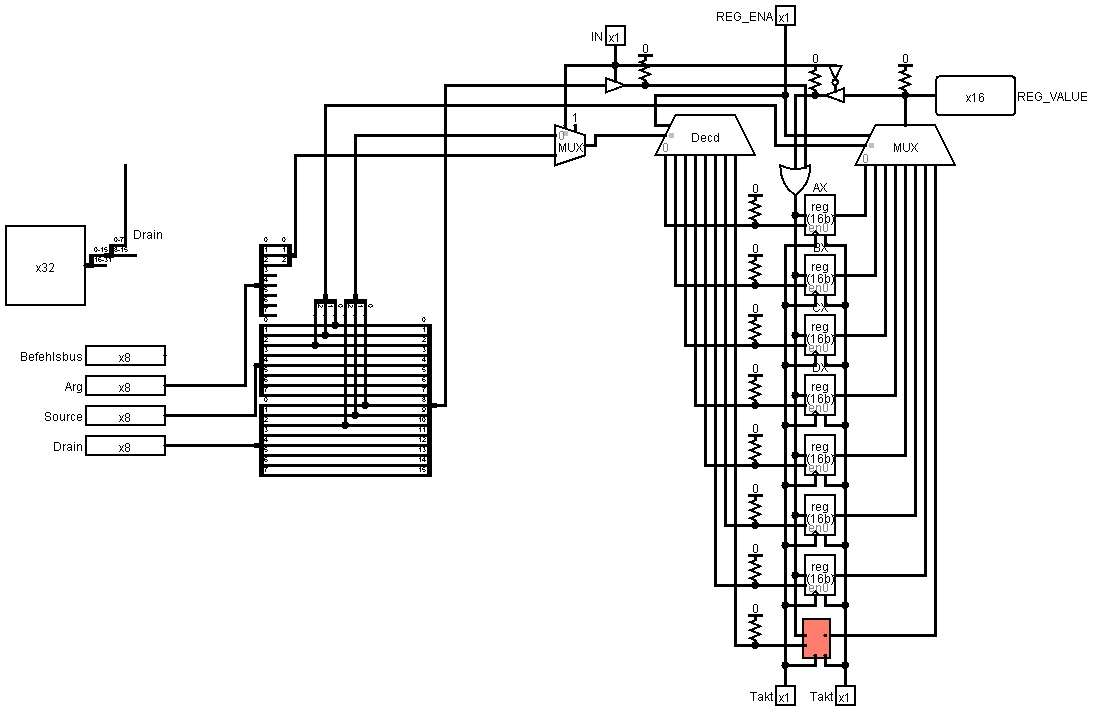
\includegraphics[scale=0.40]{circ}
\caption{Darstellung des RegisterwerkTODO}
\centering
\label{fig:register}
\end{figure}

\subsection{Register}
Register sind die schnellste Speichereinheit innerhalb einer CPU. Prozessoren besitzen eine vielfach höhere Ausführungsgeschwindigkeit als Arbeitsspeicher. Die CPU müsste ohne Register viele Taktzyklen auf Daten warten bevor sie diese verarbeiten könnte. Register bieten deshalb die Möglichkeit, sehr kleine Datenmengen mit einer sehr geringen Latenz prozessorintern lesen und schreiben zu können. Übliche Registergrößen sind 8,16,32 oder 64 Bit.\cite{mikroprozessortechnik2011} Sie werden aus Flip-Flops aufgebaut welche jeweils genau ein Bit speichern können, das heißt ein 64 Bit Register besteht aus 64 gemeinsam gesteuerten Flip-Flops.\cite{mikroprozessortechnik2011} Diese Art der Datenspeicherung hat allerdings auch einige Nachteile. So verbrauchen Register sehr viel Energie und Platz auf dem Prozessordie, es werden deshalb keine großen Speichermengen zur Verfügung gestellt. (Nachteile evtl streichen)

\subsubsection{Universalregister}
Es werden zwei Arten von Registergruppen unterschieden.In einem Universalregister kann ein Programm Werte und Variablen abspeichern.Sie stehen außerdem einem Programmierer von außen offen, das heißt er kann auf jedes Universalregister direkt zugreifen und seinen Wert verändern.

\subsubsection{Spezialregister}
Spezialregister werden von einer CPU für interne Zwecke genutzt. Oft sind in Prozessoren ähnliche Spezialregister zu finden. 

Der StackPointer(SP) ist ein Register welcher auf die aktuelle Position des Stacks im Speicher zeigt. Wenn der Befehl zu Speicherung eines Werts auf dem Stack ausgeführt wird inkrementiert die CPU automatisch, durch die interne Verschaltung des SP, den Wert des StackPointers. Dadurch zeigt das Register immer auf die nächste freie Speicheradresse im Stack.

Der InstructionPointer(IP) enthält die Adresse des nächsten Befehls im Programmspeicher der ausgeführt werden muss. Auch er wird nach der Abarbeitung eines Befehlszyklus als letzter Schritt inkrementiert. Dieses Register bietet allerdings die Möglichkeit einen anderen Wert zu laden. Das wird zur Realisierung von Sprüngen innerhalb des Programmcodes benötigt. 

Das Statusregister(SR) werden zur Ausführung von bedingten Sprunganweisungen gebraucht. Sie werden auch Flagregister genannt da die ALU, in Abhängigkeit der zuletzt ausgeführten Rechenoperation, einzelne Bit(Flags) setzen kann. Auf die einzelnen Flags und ihre Bedeutung wird im Abschnitt der ALU näher eingegangen
\subsection{Arithmetisch Logische Einheit}
\subsubsection{ALU-Konfigurationen}
%https://en.wikibooks.org/wiki/Microprocessor_Design/ALU#Example:_4-Bit_ALU
%https://en.wikibooks.org/wiki/Microprocessor_Design
\subsubsection{Arithmetische Operationen}
\subsubsection{Logische Operationen}
\subsection{Memory Management Unit(evtl)}
\subsection{Bussysteme}

\section{Speicher}
%https://de.wikipedia.org/wiki/Speicherhierarchie
\subsection{RAM/ROM}
\subsection{Stack}

\section{Befehlsausführung}
\subsection{Befehlszyklus}
\subsection{Schleifen}

\section{Besondere Ausführungsarten}
\subsection{Interrupts}
\subsection{Exceptions}
\subsection{Subroutinen}



\section{Planung und Entwurf eines Prozessors}
\subsection{Befehlsbreite}
\subsection{Befehlssatz}
\subsection{Speicher}
\subsubsection{RAM/ROM}
\subsubsection{Stack}

\section{Implementierung einer Prozessorsimulation in Logisim}
\subsection{Logisim}
\subsection{Prozessor Komponenten}
\subsection{Ausführung eines Assemblerprogrammes}

\newpage
\bibliography{Referenzen}

\end{document}
